%\documentclass{article}
\documentclass[a4paper, 12pt, oneside]{book} % Uses the book template for quick start, but scrbook may be better because it is more flexible
\usepackage{inputenc}
\emergencystretch=2em
\usepackage[breaklinks]{hyperref}
\hypersetup{
    colorlinks=true,
    linkcolor=blue,
    filecolor=magenta,      
    urlcolor=magenta,
    citecolor=black}
\usepackage[english]{babel}
%\usepackage{biblatex}
\usepackage[backend=biber, style=apa]{biblatex}
\setlength\bibitemsep{\baselineskip}
\usepackage{svg}
\usepackage{graphicx}
\usepackage[labelfont=bf]{caption}
\usepackage{booktabs}
\usepackage{caption}
\usepackage{subcaption}
\usepackage[left]{lineno} % For line numbers
%\renewcommand{\baselinestretch}{2.0}
%\linenumbers
\usepackage[T1]{fontenc} % Include italic fonts
\usepackage{geometry} % Page margins
\usepackage{titling} % Title page container
\usepackage{wrapfig} % Picture container
\usepackage{titlesec} % Remove chapter header
\renewcommand{\familydefault}{\sfdefault} % Set default f

% COLORS
%\usepackage{xcolor} 
%\usepackage{soul}
%\definecolor{color1}{HTML}{a5ddd0}
%\definecolor{color2}{HTML}{00441b}
%\sethlcolor{color1}\hl{Its trunk bears spikes to deter attacks by animals. <0.35> }
%\sethlcolor{color2}\hl{Branches usually in whorls of 3. <1.0> }

\addbibresource{references.bib}
% Note: Fill these in with correct data, they are used throughout the document
\title{A Step Towards Explainable AI: Infer Species Names Based on Partial Descriptions in Natural Language}
\author{Robert van de Vlasakker}
% This can be left as-is to automatically update
\date{\today}
\geometry{top=2.25cm, 
            bottom=2.91cm,
            inner=2.91cm,
            outer=2.91cm,
            foot=0cm,
            includeheadfoot} % First page margins
\titleformat{\chapter}[display]
  {\normalfont\bfseries}{}{0pt}{\Large}

\begin{document}
 \begin{titlingpage}


  %\newgeometry{top=1.25cm,bottom=1.25cm,inner=0.66cm,outer=0.53cm,foot=1.19cm,includeheadfoot} % Subsequent page margins
  % Note: this uses the MS Word template margins, you might want to increase them a bit for printing (e.g. inner=1.91cm,outer=1.91cm)
  \thispagestyle{empty}
  
  \begin{center}
  {\bfseries \Large \thetitle}
  \newline
  \newline
  \newline
  \newline
  %{\bfseries \itshape Subtitle}\vspace{2.7cm}
  
  {\Large \theauthor}\vspace{0.8cm}
  
  {Registration number 920523897020}\vspace{2.5cm}
  
  {\large \underline{Supervisors}:}\vspace{1.1cm}
  
  {Diego Marcos}
  
  {Ioannis Athanasiadis}\vspace{3.0cm}
  
  %{A thesis submitted in partial fulfilment of the degree of Master of Science}
  
  %{at Wageningen University and Research Centre,}
  
  %{The Netherlands.}\vspace{2.7cm}
  \end{center}
  
  \begin{center}
    {\thedate}
  
    {Wageningen, The Netherlands}
  \end{center}\vspace{6cm}

    Thesis code number: GRS-80400
  
    Thesis Report: Proposal
  
    {Wageningen University and Research Centre}
  
    {Laboratory of Geo-Information Science and Remote Sensing}
 \end{titlingpage}
\graphicspath{ {./figures/} }

\renewcommand{\thesection}{\arabic{section}}
\section{Introduction}
Estimated is that 50\% of the species are yet to be discovered, and many species will go extinct before ever being described \autocite{lees_species_2015}.
Scalable technologies that can help monitor diversity and help discover new species are more needed than ever.
Deep neural networks (DNNs) can help discover new species, automate and speed up this process \autocite{van_horn_inaturalist_2018}.
However, DNNs are quite rigid, and their black-box behaviour could raise issues as it hampers the trustworthiness of the models \autocite{carvalho_machine_2019}.
It is essential to get more insights into the reasoning of a deep learning model in sensitive fields like taxonomy.
This way, we can learn a DNN to reason like an experienced taxonomist when describing existing and new species.

Deep neural networks (DNNs) allow for remarkable performance in applications: from the automatic classification of text and images, natural language processing (NLP), to reinforcement learning.
DNNs outperform most classic machine learning approaches \autocite{he_delving_2015, brown_language_2020}.
The key to their success is end-to-end training.
Unlike classic machine learning models, deep learning models can automatically extract features needed for detection or classification.
Domain knowledge, in combination with careful engineering to extract the necessary features for the detection or classification, is no longer needed \autocite{lecun_deep_2015}.
However, end-to-end training also results in DNNs that are rigid, difficult to interpret and explain.
To extract the features from the input data, deep learning models use multiple neurons that take the input, process it to a slightly more abstract representation and pass it through the next layer of neurons \autocite{schmidhuber_deep_2015}.
Provided enough layers are stacked upon each other, very complex features can be extracted and correctly detected or classified by such a network.

Because the network's parameters are updated based on its input data, the reasoning of DNNs remains challenging to understand \autocite{li_interpretable_2021, losch_interpretability_2019}, and they do not perform well on long-tailed datasets, like most real-world datasets \autocite{van_horn_inaturalist_2018}.
Stacking multiple layers of neurons on top of each other often results in millions of parameters, and all of these neurons use non-linear activation functions that decrease the interpretability of the network.
In long-tailed datasets, the parameters are not well optimised for less represented classes as the neurons cannot extract the necessary features.
While this automatic feature extraction is very convenient, it will become difficult to track models' reasons, and it can hamper performance.

\begin{figure} [h]
    \centering
    \vspace{0cm}
    \makebox[\textwidth][c]{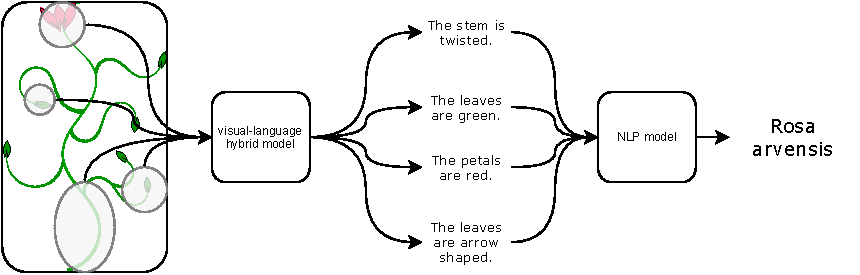
\includegraphics[width=1.25\textwidth]{intrduction_overview.pdf}}
    \caption{The proposed architecture by \textcite{ishikawa_contextual_2021} for species classification. The model input is an image. The first model will describe the attributes present in the image in natural language. The second model will take the output of the first model and will make a prediction. The intermediate results remain interpretable by using natural language.}
    \label{fig:intro}
\end{figure}

A more explainable, less rigid, artificial intelligence (AI) might be created by extending the concept of the semantic bottleneck layer from \textcite{ishikawa_contextual_2021} and splitting a regular convolution neural network (CNN) for image classification into two separate models that communicate using natural language.
The first model will describe species features present in the image, and the second model will take these descriptions and tries to infer the species (see Figure \ref{fig:intro}).
This way, DNNs reasonings for species classification can be tracked, mistakes can be spotted, and the models' performance can be improved.


Many studies have already stipulated the importance of biodiversity for human life \autocite{pimentel_economic_1997, gowdy_value_1997, raffaelli_links_2010, joppa_biodiversity_2011, pimm_how_2018}.
With the current extinction rate, over 50\% of the species will be gone before ever discovered \autocite{lees_species_2015}.
Protecting biodiversity is now more needed than ever.
However, we cannot conserve undiscovered species; we first need to describe them to protect them \autocite{joppa_biodiversity_2011}.
DNNs can help discover new species and speed up this identification process \autocite{van_horn_inaturalist_2018}.
However, many species look alike.
They are difficult to distinguish and are easily miss-classified, especially with less abundant species.
We need a better understanding of how a DNN identifies and classifies species. 
This way, a less rigid DNN can be created, results of the DNN can be interpreted more easily, and the results can be improved.

Different algorithms and techniques have been proposed to increase the interpretability of the models.
Common approaches are feature reduction algorithms \autocite{ribeiro_why_2016}, inference of training sample contribution \autocite{koh_understanding_2020}, adding jittering to test samples and see how the prediction changes \autocite{li_understanding_2017} and decomposition and partial derivatives techniques \autocite{samek_explainable_2017}.
These algorithms and techniques all rely on posthoc explanations; they try to interpret an already trained DNN and explain its decisions a posteriori.
They try to identify important features via attributions \autocite{zintgraf_visualizing_2017, selvaraju_grad-cam_2017} or assign meaning to features \autocite{fleet_visualizing_2014}.
While some advances have been made in model understanding, giant leaps forward in the field of explainable AI remain limited \autocite{lipton_mythos_2017, li_interpretable_2021}.
These approaches might explain some of the inner workings of a DNN, but they do not help reason a DNN like a taxonomist, the models remain rigid, and the intermediate results still remain challenging to interpret. 

An a priori approach entails designing an architecture network with a semantic bottleneck layer that is interpretable for humans \autocite{bucher_semantic_2019}. 
\textcite{ishikawa_contextual_2021} extended this bottleneck layer architecture by training a model that first learns the intermediate results.
First, a model is trained that can predict semantic attributes.
The second model will take the intermediate results to make a final prediction.
By using their architecture, a less rigid, more explainable AI for species classification might be created.

The first model will be a visual-language model that extracts the species attributes from an image and describes its results in natural language. 
This vision hybrid model will be based on the researches of \textcite{radford_learning_2021} and \textcite{huang_interpretable_2020}.
Their findings allow the first model to learn to extract information from images by looking at raw text data that comes with image captions and describe objects present in those images.
This visual-language hybrid model will describe learned species attributes and use zero-shot learning to describe unseen (new) distinctive species attributes.
By first describing traits, less abundant species can benefit from more abundant species if they share common traits.
The second model is a pure natural language processing (NLP) model that takes the partial descriptions and infer the species.
This way, a models reasoning for species predictions might be tracked by investigating the intermediate results \autocite{ishikawa_contextual_2021} and the final model results will be less rigid.

For the training of both models, an extensive labelled database with species and their descriptions is needed. 
Unfortunately, such a database does not yet exist and needs to be created for this research to happen.
This dataset needs as many unique descriptions as possible for each species, so for both a taxonomist and the NLP model, it would be possible to infer the species name based on provided descriptions.
The NLP model needs to make predictions on partial descriptions, but in the meantime, it should be clear which parts of the description data is used to make to prediction so the reasoning can be evaluated.
This research will focus on creating and curating the dataset containing species and their descriptions and the training and evaluation of the NLP model.
\newpage
\section{Approach}

In Figure \ref{fig:workflow} a simplified version of the workflow can be found.
This chapter will give a detailed description of the steps.

\begin{figure} [t]
    \centering
    \vspace{-2cm}
    \makebox[\textwidth][c]{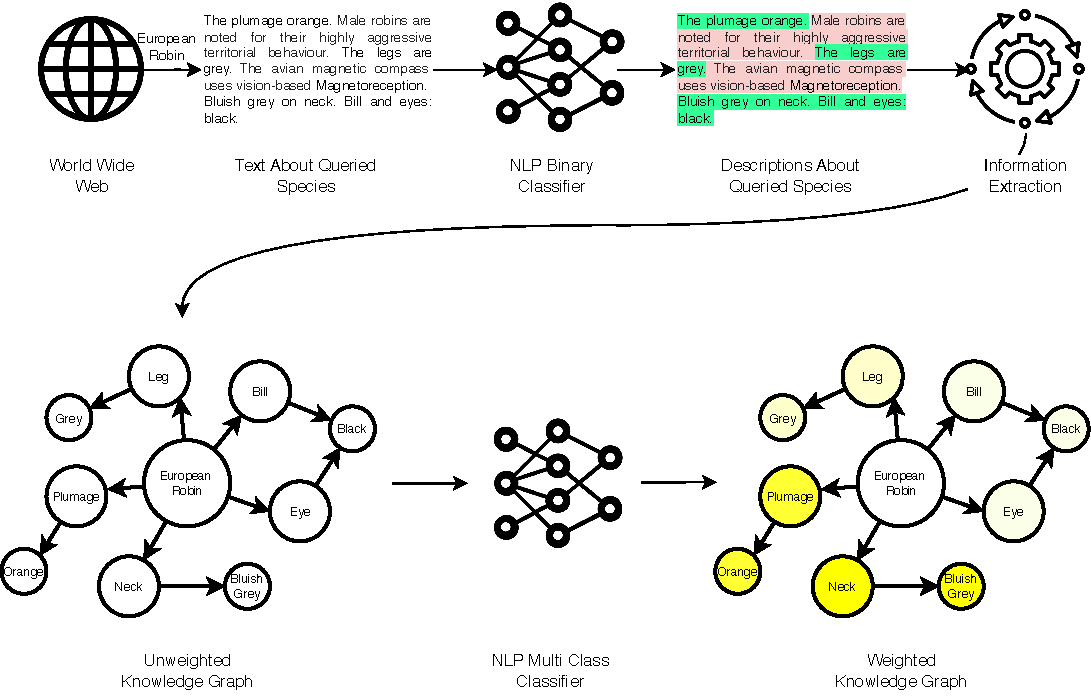
\includegraphics[width=1.25\textwidth]{workflow.pdf}}
    \caption{A simplified workflow. Text data is used to train a model to recognize species description. In this case the paragraph titles are used as labels. The model is deployed in a web crawler that searches the web for species descriptions. These data are then used to train the NLP model independently of the visual-language hybrid model. The NLP model will focus on important words to recognise the species.}
    \label{fig:workflow}
\end{figure}

\subsection{Creating an Extensive Dataset}
The World Wide Web also has potentially an endless amount of species descriptions available.
This makes the internet suitable for harvesting training data.
However, description sentences can be theoretically limitless, e.g. for a Brown Bear description text could be: "The fur is brown", "The brown bear has brown fur".
Sentences can have a more difficult semantic, e.g. "The fur of the Brown bear is similar to that of the Grizzly bear".
A classic machine learning approach that requires a rule-based match system for sentence classification is not possible. 
We trained a DNN that can classify text into description or non-description.
To properly train a deep learning model that can classify text data, a large, accurate and consistent labelled dataset is needed \autocite{munappy_data_2019}.

\subsubsection{Training Data}
We create this dataset by scraping web pages from structured sources.
These sources (Wikipedia, Plant of the World Online (PoWO), Birds of the Word(BoW)), have a rich scholarly content about species.
These websites divide their information into paragraphs such as "Introduction", "Appearance", "Characteristics", "Habit".
These paragraph titles are used as labels and the text inside is used as data.
In our case we stored text from paragraphs with titles like:  "Introduction" and "Habit" as negative values and "Introduction" and "Appearance" as positive values, making this a two class classification problem. 
Wikipedia is also used to gather additional negative values, as this Wikipedia also contains a lot of pages without any species information.
This allows the model to better classify text not related to species descriptions.


%BERT models use two specials tokens.
%This first token is always \verb|[CLS]|, which stands for "Classification".
%Using \verb|[CLS]|, the model knows the sequence is used for classification.
%The second token is \verb|[SEP]|, which stand for "Separation". 

\subsubsection{BERT for Classification}
Using a pre-trained model can provide significantly improvements over models trained from scratch \autocite{mikolov_distributed_2013}.
The use of a pre-trained model is called transfer learning and could speed up the training process and increase the accuracy of the deep learning model.
The Bidirectional Encoder Representations from Transformers (BERT) by \textcite{devlin_bert_2019} is already trained on a large corpus of English words and can be used freely.
As a base, We used a distilled version of BERT \autocite{devlin_bert_2019}, called distilBERT \autocite{sanh_distilbert_2020}. 
This version is 60\% faster, has 40\% less parameters and still reaches 97\% on general language understanding.
\textcite{sun_how_2020} already investigated how to fine-tune BERT for text classification and we used their findings in this research.

BERT can be fine-tuned further by updating the inner parameters of BERT during training. 
This can be useful if BERT is utilised in the non-general domain \autocite{devlin_bert_2019, sun_how_2020, sanh_distilbert_2020}, which is the case with description data.
However, we decided not to fine-tune the inner workings of BERT for two reasons: 
(1) We used additional Wikipedia to increase the text data with negatives values.
These random Wikipedia pages are highly likely to contain information from the general
domain, resulting in a  data distribution close(r) to the general domain.
(2) A two class-classification problem is a relatively simple task, updating the inner parameters during training cost additional time and computing power, while only resulting a small accuracy increase.

Like \textcite{sun_how_2020} we first fit a fully connected linear layer with an input size of 768 and an output size of 512 on top of the BERT architecture. 
This linear layer is followed by a dropout layer (0.1) to enable some regularization.
The next fully connected linear layer has a input size of 512 and an output size of 2, as we are predicting two classes.
The final activation layer is a log-likelihood (log-softmax) activation function.
The log-softmax will slightly increase the error factor of the model, punishing mistakes a bit higher.
By taking the exponent, the standard likelihood (softmax) probabilities can be computes.

Instead of a cross entropy loss, we use a loss from \textcite{reed_training_2015}:
\begin{equation} \label{eq:softloss}
 SoftLoss(q, t) = \sum_{k=1}^{L}[\beta t _k + (1- \beta )q _k]log(q _k)
\end{equation}
This allows the model for semi-supervised learning.
Not all data will be labelled correctly as the paragraph titles are used as labels.
E.g. some species description might be located in the paragraph "Introduction" and some general information might be in the paragraph "Characteristics".
This softloss is based on a normal cross entropy loss.
In equation \ref{eq:softloss}, \(q\) is directly used to calculate regression targets for each batch.
If the predefined \(\beta\) reaches a threshold, the prediction is treated as correct and the loss is calculated accordingly.
Consider the text "The European robin is red-breasted with distinctive eyes.".
This text is likely to be found in a paragraph about descriptions.
However, the text can also occur in the introduction paragraph about an European robin or it could be part of an image caption of an entirely different paragraph. 
In second case the text will be miss classified. 
By implementing the semi-supervised loss function of \textcite{reed_training_2015}, this will be prevented to a certain extent.
If the model prediction reaches the set threshold, the prediction is seen a description label, but if the model prediction are below the threshold, the loss will be calculated accordingly.
In this thesis we use a \(\beta\) of 0.80. 

To prepare the text spans, we use the tokenizer of \textcite{wolf_huggingfaces_2020}.
The used BERT architecture can only process up to 512 token at once \autocite{sanh_distilbert_2020, devlin_bert_2019}.
Most tokenizers will truncate text spans larger then 512 tokens as most text information is in the beginning (head-encoding), end (tail-encoding) or beginning and end (head+tail-encoding).
We decide not truncated the text.
Instead we randomly split the text into text spans with a minimum of 10 words and a maximum of 512 words.
We hypothesised that the model might be better in recognising shorter description spans by splitting the raw spans.  
This way we enlarge the dataset, prevent loosing information with truncating spans larger then 512 tokens. 
We use a minimum of 10 words to prevent the model fixating on specific words.
The tokenizer of \textcite{wolf_huggingfaces_2020} returns a Python dictionary with the input ID's and the attention mask of the text.
E.g. by tokenizing the text "This is a test.", the tokenizer returns the following:
\verb|{'input_ids': [101, 2023, 2003, 1037, 3231, 1012, 102]|, 
\verb|'attention_mask': [1, 1, 1, 1, 1, 1, 1]}|.
\verb|[101]| indicates the start of a sequence and \verb|[102]| indicates the end of a sequence.
During the training the text is also padded to the maximum of 512 tokens and the attention masks are randomised between 0 and 1.


\subsubsection{Training BERT for Text Classification}
We train the model on a Google Colab instance.
We used the Adam optimiser \autocite{kingma_adam_2017}.
The Adam optimiser has shown good performance when fine-tuning BERT for text classification \autocite{you_large_2020}.
The hyperparameters were set based on the paper of \textcite{sun_how_2020}.
The learning rate was set to 3e-5 and the batch size was set to 32.
During the training the gradients are clipped to prevent the gradients from becoming to large.
The model was trained for 35 epochs.

\subsubsection{Evaluation BERT for Text Classification}
As the dataset is will be unbalanced it will be evaluated with a precision-recall summary, receiver operating characteristics (ROC) and a precision-recall curve.
The precision-recall summary and curves give more reliable results with an unbalanced dataset.
When the model reaches an f1-score of at least 0.9, the model is tested on two additional left out databases, the \href{http://www.llifle.com/}{LLifle} dataset and the \href{https://www.worldagroforestry.org/}{AgroForestry} dataset.
The data will be first cleaned (e.g. references, footnotes) and will be split into sentences using a senticizer from \textcite{honnibal_spacy_2020}.
The text paragraphs are again used as labels. 
To correct for missclassified labels, a modified version of Equation \ref{eq:softloss} is used to calculated the precision-recall report, see Equation \ref{eq:softloss_ifthen} for the label correction.
\begin{equation} \label{eq:softloss_ifthen}
(\hat{\gamma}^{(i)} >= \beta \rightarrow \hat{\gamma}^{(i)} = \gamma^{(i)}) \wedge ( \leftharpoondown \hat{\gamma}^{(i)} = \hat{\gamma}^{(i)})
\end{equation}
This is the loss function from \textcite{reed_training_2015}, only notated in an If-Then statement to compensate for the miss labelled sentences of the external datasets, as losses are no longer calculated in these cases.

\subsubsection{Web Crawler Deployment}
We deploy the classification model in a web crawler.
This web crawler can automatically query search engines with a predefined list of birds and plants.
The list for plants is based on the \href{https://www.ipni.org/}{International Plant Name Index} (IPNI) and the list for birds is based on the database of \href{https://birdsoftheworld.org/bow/home}{Birds of the World} (BoW).
The IPNI database contains over 1,3 million plant species and the BoW database contains over ten thousand birds.
The plant species are sorted based on their number of descriptions in the PoWO dataset.
Plant species with a description have a higher chance of being described somewhere else on the web as the PoWO dataset is closely linked to the IPNI database.

The web crawler with query the search engines resulting in a list URLs with possible species descriptions.
We use five different ways of constructing a query:
\begin{itemize}
    \item "Species"
    \item "Species+description"
    \item "Species+diagnosis"
    \item "Species+attributes"
    \item "Species+captions"
\end{itemize}
The URL list is checked for duplicates as this is computationally less expense than calculating the cosine similarity (see Section \ref{Sentence Similarity} about Sentence Similarity).
The URLs are checked for text data without any markup, like raw text data and PDF files.
Finally the header of the URL is checked against the queried species to make sure that the page really contains information about the queried species.

If the URL meets all criteria, the raw text is retrieved and broken down into single sentences. 
This makes sure the descriptions will be stored as much as possible per unique species trait.
The text is cleaned using several regular expressions.
Every sentence is checked against the train description classifier.
If a description is recognised by the model, the sentence is stored.

\subsubsection{Sentence Similarity} \label{Sentence Similarity}
There is a change that different web pages use the a common source for describing a species.
By checking for similar sentence within the same species we make sure the same sentence is not appended twice to the dataset and the train and test set are completely disjoint.
Like \textcite{reimers_sentence-bert_2019} we use the last hidden state of BERT (distilBERT) in our case and compute the cosine similarity to measure the distance between text spans.
Fortunately, this last hidden state is the output of a base BERT architecture.
However, the last hidden state output contain a matrix of 512 x 768. 
It is not feasibly to compute the cosine similarity distance for multiple matrices of this size.
By using a mean-pooling operation we create a vector of size 768 for every text span and compute the cosine distance for these text spans.

We first create a new dictionary that corresponds to the dictionary initialised by the tokenizer, \verb|{'input_ids': [], 'attention_mask': []}|.
We tokenize all the sentences we are comparing and append the tokens and masking to the correct key.
After all the sentences have been processed, we reformat the dictionary into a single tensor and push it trough the model.
This will result in a tensor of the number of sentences times 512 times 768. 
We sum the matrix along the first axis, resulting in a matrix.
The size of this matrix is the number of sentences time 768.
Each sentence is represented by a vector of size 768
Finally we calculate the cosine similarity between the sentences and drop sentences that exceed the threshold of 0.99.

\subsubsection{Storage Preprocessing}
Before storage the sentences are processed.
Description sentences often name the species in the description, e.g. "Fagus sylvatica is a large tree, capable of reaching heights of up to 50 m (160 ft) tall." (source: \href{https://en.wikipedia.org/wiki/Fagus_sylvatica}{Wikipedia/wiki/Fagus\_sylvatica}).
Species names are replaced by the word "the species". 
In the example above the sentence is stored as: "The species is a large tree, capable of reaching heights of up to 50 m (160 ft) tall."
This way the NLP model will not have access to (parts of) the labels of the input data.

Some databases store their description as one long sentence,

\subsection{Inferring Species}
\subsection{Retrieving Keywords}


\newpage
\section{Results}
\subsection{Extensive dataset}
\subsubsection{Description Classification}

\begin{figure} [t]
    \centering
    \vspace{0cm}
    \makebox[\textwidth][c]{\includesvg[inkscapelatex=false, width=1.25\textwidth]{histogram_text_length.svg}}
    \caption{The text length distribution before tokenization. The text spans are randomly split into chunks between 10 words and their length, with a maximum of 512 words to prevent truncation. Text spans with a length below 10 words are not split, resulting in some text lengths below 10. There are some text length with the maximum value of 512. This count is barely visible in the plot, so the x-axis limit is set to a max text length of 250.}
    \label{fig:text_length_distribution}
\end{figure}

Scraping the structured sources and using their paragraph titles resulted in 1,086,576 samples.
Each sample consists of a tuple, containing the label (0/1) and the text span.
The text spans of the samples are randomly split into chunk resulting in 1,867,932 tuples with label and text.
451,862 tuples have a label that corresponds to a description (label 1) and 1,416,070 tuples have a label that correspond to something different (label 0).
In Figure \ref{fig:text_length_distribution} the distribution after splitting the original samples in random chunks can be found.

The test data is evaluated with a precision-recall plot.
This plot can be found in Table \ref{tab:precision_recall_descriptionsmodel}.
The model seems to perform excellent on both classes.
The model reaches an high precision, recall and f1-score for both the "Non-Description" and "Description" class.

\begin{table}[h]
\centering
\caption{The precision-recall report for the test set for the binary classification model on descriptions. 10\% of the data is left out for testing. The model is trained for 35 epochs.}
\label{tab:precision_recall_descriptionsmodel}
\begin{tabular}{@{}lcccr@{}}
\cmidrule(l){2-5}
 & \multicolumn{1}{l}{Precision} & \multicolumn{1}{l}{Recall} & \multicolumn{1}{l}{f1-score} & \multicolumn{1}{l}{Support} \\ \midrule
Non-Description  & 0.98 & 0.99 & 0.99 & 167,955 \\
Description      & 0.97 & 0.95 & 0.96 & 57,864  \\ \midrule
Accuracy         &      &      & 0.98 & 225,819 \\
Macro Average    & 0.98 & 0.97 & 0.98 & 225,819 \\
Weighted Average & 0.98 & 0.98 & 0.98 & 225,819 \\ \bottomrule
\end{tabular}
\end{table}

\noindent
The corresponding ROC and precision-recall curve can be found in Figure \ref{fig:ROC_test} and Figure \ref{fig:precision_recall_curve_test}.
Both the ROC curve area and the AP reaches 99\% indicating the binary classifier separates both classes very well.

\begin{figure} [h]
     \centering
     \begin{subfigure}[b]{0.49\textwidth}
         \centering
         %\hspace{-1.0cm}
         \includesvg[inkscapelatex=false, width=\textwidth]{AUC-ROC.svg}
         \caption{The Receiver Operating Characteristics (ROC) for the test data.}
         \label{fig:ROC_test}
     \end{subfigure}
     \hfill
     \begin{subfigure}[b]{0.49\textwidth}
         \centering
         %\hspace{-0.5cm}
         \includesvg[inkscapelatex=false, width=\textwidth]{precision_recall_plot.svg}
         \caption{The Precision-Recall curve for the test data.}
         \label{fig:precision_recall_curve_test}
     \end{subfigure}
     \caption{The ROC and the precision-recall curve for the left out test set. The models seems to perform excellent in both cases. The model is evaluated on a test set that contains 10\% of the data. The Area Under the Curve (AUC) reaches 99\% and the the Average Precision (AP) reaches 99\%.}
\end{figure}
The model is evaluated on two additional datasets, the \href{http://www.llifle.com/}{LLifle} dataset and the  \href{https://www.worldagroforestry.org/}{AgroForestry} dataset
These datasets are completely left out of the training/testing fase of the model.
Together, these dataset contain 17,204 tuples.
771 text spans correspond to a description, and 16,433 text spans corresponds to something different.
After the text has been cleaned and split into sentences there are 74,836 tuples.
There are 8,590 tuples with a descriptions sentence and 66,246 tuples that contain a sentence describing something different.
In Table \ref{tab:precision_recall_descriptionsmodel_external} the precision-recall summary for the external datasets can be found.
The corresponding ROC and precision-recall curve can be found in \ref{fig:ROC_test_external} and \ref{fig:precision_recall_curve_test_external}.
The overall performance of the classifier on the external datasets is excellent. 
The ROC curve area reaches 99\%, the same performance as on the test set (visually it seems a bit less).
The AP reaches 96\%.
\begin{table}[h]
    \centering
    \caption{The precision-recall report for the binary classification model tested on two external datasets (LLifle and AgroForestry).}
    \label{tab:precision_recall_descriptionsmodel_external}
    \begin{tabular}{@{}lcccr@{}}
    \cmidrule(l){2-5}
     & \multicolumn{1}{l}{Precision} & \multicolumn{1}{l}{Recall} & \multicolumn{1}{l}{f1-score} & \multicolumn{1}{l}{Support} \\ \midrule
    Non-Description  & 0.99 & 0.98 & 0.98 & 66,051 \\
    Description      & 0.83 & 0.90 & 0.86 & 8,785  \\ \midrule
    Accuracy         &      &      & 0.97 & 74,836 \\
    Macro Average    & 0.91 & 0.94 & 0.92 & 74,836 \\
    Weighted Average & 0.97 & 0.97 & 0.97 & 74,836 \\ \bottomrule
    \end{tabular}
\end{table}

\begin{figure} [h]
     \centering
     \begin{subfigure}[b]{0.49\textwidth}
         \centering
         %\hspace{-1.0cm}
         \includesvg[inkscapelatex=false, width=\textwidth]{AUC-ROC_external.svg}
         \caption{The Receiver Operating Characteristics (ROC) for the left out data.}
         \label{fig:ROC_test_external}
     \end{subfigure}
     \hfill
     \begin{subfigure}[b]{0.49\textwidth}
         \centering
         %\hspace{-0.5cm}
         \includesvg[inkscapelatex=false, width=\textwidth]{precision_recall_plot_external.svg}
         \caption{The Precision-Recall curve for the left out data.}
         \label{fig:precision_recall_curve_test_external}
     \end{subfigure}
     \caption{The ROC and the precision-recall curve for the left out external datasets. The models seems to perform reasonable in both cases. The Area Under the Curve (AUC) reaches 99\% and the the Average Precision (AP) reaches 96\%. In both plots the blue dashed line indicates a baseline classifier.}
\end{figure}

\subsubsection{Web Crawler}
\subsubsection{Sentence Similarity}

\subsection{Species Classification}
\subsection{Key Words}

\printbibliography
\end{document}